\chapter{Metodologia}
\label{chap:metodologia}

Esta seção descreve o planejamento metodológico que será executado na segunda
etapa deste trabalho (TCC2). A pesquisa classifica-se como exploratória e
descritiva, utilizando uma abordagem mista (qualitativa e quantitativa) para
compreender a fundo o fenômeno estudado \cite{creswell2010projeto}. O objetivo
é garantir que os métodos escolhidos respondam diretamente à hipótese de que o
protagonismo do aluno e a integração de saberes geram soluções de software mais
assertivas.

\begin{figure}[h!]
	\centering
	\Caption{\label{fig:fluxo-metodologico} Etapas do Processo Metodológico.}
	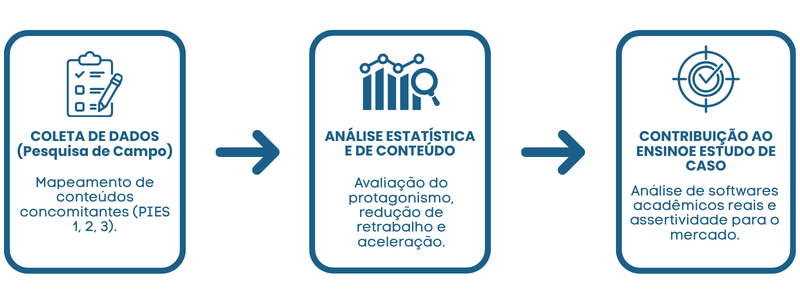
\includegraphics[width=0.9\textwidth]{figuras/metodologia_pesquisa_academica.png}
	\Fonte{Elaborado pelo autor.}
\end{figure}

Para garantir que todos os objetivos específicos sejam alcançados de forma
coerente, o processo de pesquisa foi dividido em 3 etapas sequenciais.
Esse fluxo metodológico guiará a execução do TCC2, conectando a base teórica
com a coleta e análise de dados reais.

A Figura \ref{fig:fluxo-metodologico} ilustra visualmente o fluxo dessas
etapas e resume o detalhamento técnico de cada passo que será adotado.

\newpage
\section{Coleta de Dados (Pesquisa de Campo)}\label{sec:coleta-de-dados}
Para coletar dados e métricas reais sobre a percepção dos estudantes a respeito
do uso conjunto de múltiplas áreas do conhecimento, será aplicado o método de
Survey (Pesquisa de Levantamento) \cite{gil2008metodos}.

Serão desenvolvidos três formulários digitais direcionados especificamente aos
alunos que cursam ou cursaram PIES 1, PIES 2 e PIES 3. As perguntas utilizarão
a Escala Likert de 5 pontos \cite{joshi2015likert}, permitindo quantificar o
nível de concordância dos alunos sobre o impacto das disciplinas complementares
(como Banco de Dados, Web e UX) no sucesso dos seus projetos práticos. Além
disso, o formulário conterá perguntas abertas para identificar as barreiras que
eles enfrentam com a fragmentação do ensino.

\section{Análise e Avaliação dos Resultados}\label{sec:analise-e-avaliacao-dos-resultados}
Com os dados coletados, a pesquisa passará para a etapa de análise mista. As
respostas quantitativas da Escala Likert passarão por uma Análise Estatística
Descritiva, gerando gráficos que demonstrarão o impacto das metodologias ativas
na redução do retrabalho e na aceleração do desenvolvimento. Já as respostas
abertas passarão por uma Análise de Conteúdo \cite{bardin2016analise} para
categorizar as principais dificuldades relatadas pelos estudantes.

Por fim, para analisar se a integração de diferentes saberes resultou na
entrega de softwares mais assertivos para o mercado, será utilizado o método de
Estudo de Caso \cite{yin2015estudo}. Serão selecionados projetos reais
desenvolvidos pelos alunos nas disciplinas de PIES. A avaliação focará em
cruzar as respostas dos alunos com a qualidade técnica do software entregue,
provando (ou refutando) a hipótese de que o protagonismo estudantil e a
integração de matérias geram inovação prática.